% +++
% latex="texfot lualatex-dev"
% +++
\documentclass[
	paper=A4,
	tbtags,
	DVI=14,
]{scrartcl}

\usepackage{luatexja,luatexja-adjust}
\usepackage[no-math,match]{luatexja-fontspec}
\ltjsetparameter{jacharrange={-2,-3,-8}}

%\usepackage[x-1a]{pdfx}

\usepackage{xcolor,hyperref}
%\selectcolormodel{cmyk}
\hypersetup{unicode,colorlinks}
\hypersetup{linkcolor=blue,urlcolor=teal,citecolor=olive}
% \hypersetup{linkcolor=black,urlcolor=black,citecolor=black}

\usepackage{pxrubrica}
\usepackage{autobreak}
\usepackage{tikz,pgfplots,tcolorbox}
\usetikzlibrary{calc}
\pgfplotsset{compat=1.16}

\usepackage[version=4,arrows=pgf]{mhchem}
\mhchemoptions{textfontcommand=\sffamily,mathfontcommand=\mathsf}
\newcommand*\cec[1]{\cesplit{{\,\ }{\0}}{#1}}

\usepackage{array,booktabs,tabularray}
\SetTblrDefault{rowsep=2pt}
\UseTblrLibrary{booktabs}

\usepackage{multicol}
\usepackage{subcaption}

\usepackage[loadonly,]{enumitem}
\newlist{desc}{description}{5}
\setlist[desc]{labelindent=2\zw,labelsep*=1\zw,labelwidth=3\zw}
\newlist{enu}{enumerate}{5}
\setlist[enu]{label*=\arabic*.}

\usepackage{epmaketitle} %https://github.com/matryo-sika/epmaketitle

\usepackage[style=phys,biblabel=brackets,]{biblatex}
\addbibresource{ref.bib}

\usepackage[osf]{newpxtext}\usepackage{classico}
\usepackage[nowidering]{yhmath}
\usepackage{newpxmath,amsmath,mathtools,mleftright}
\usepackage[T1]{fontenc}
\usepackage[notrig,italicdiff]{physics}
\mleftright

\ltjenableadjust[lineend=extended,priority=true,profile=true,linestep=true]

\usepackage[scr=boondoxo,frak=pxtx,bb=mth]{mathalfa}
\DeclareMathAlphabet{\mathnormal}{T1}{pplx}{m}{it}
\DeclareMathAlphabet{\mathrm}{T1}{pplx}{m}{n}
\DeclareMathAlphabet{\mathit}{T1}{pplx}{m}{it}
\DeclareMathAlphabet{\mathtt}{T1}{lmtt}{m}{n}
\DeclareMathAlphabet{\mathsf}{T1}{kurier}{m}{n}
\DeclareMathAlphabet{\mathbsf}{T1}{kurier}{b}{n}
\DeclareMathAlphabet{\mathbold}{T1}{pplx}{b}{it}
\DeclareMathAlphabet{\mathbf}{T1}{pplx}{b}{n}
\DeclareMathAlphabet{\mathscr}{U}{BOONDOX-calo}{m}{n}
\DeclareMathAlphabet{\mathbscr}{U}{BOONDOX-calo}{b}{n}
%\DeclareMathAlphabet{\mathcal}{OT1}{eusm10}{m}{n}
%\DeclareMathAlphabet{\mathbcal}{OT1}{eusm10}{b}{n}
\DeclareMathAlphabet{\mathfrak}{OT1}{tx-frak}{m}{n}
\DeclareMathAlphabet{\mathbfrak}{OT1}{tx-frak}{b}{n}
\DeclareMathAlphabet{\mathbb}{U}{dsss}{m}{n}
\DeclareSymbolFont{operators}{T1}{uop}{m}{n}

\DeclareSymbolFont{numbers}{T1}{pplx}{m}{n}
\DeclareMathSymbol{0}\mathalpha{numbers}{`0}
\DeclareMathSymbol{1}\mathalpha{numbers}{`1}
\DeclareMathSymbol{2}\mathalpha{numbers}{`2}
\DeclareMathSymbol{3}\mathalpha{numbers}{`3}
\DeclareMathSymbol{4}\mathalpha{numbers}{`4}
\DeclareMathSymbol{5}\mathalpha{numbers}{`5}
\DeclareMathSymbol{6}\mathalpha{numbers}{`6}
\DeclareMathSymbol{7}\mathalpha{numbers}{`7}
\DeclareMathSymbol{8}\mathalpha{numbers}{`8}
\DeclareMathSymbol{9}\mathalpha{numbers}{`9}

\DeclareFontFamily{U}{mathastro}{}
\DeclareFontShape{U}{mathastro}{m}{n}{<->mathastrotest10}{}
\DeclareSymbolFont{astro}{U}{mathastro}{m}{n}
\DeclareMathSymbol\Sun\mathord{astro}{'300}
\DeclareMathSymbol\Mercury\mathord{astro}{'301}
\DeclareMathSymbol\Venus\mathord{astro}{'302}
\DeclareMathSymbol\Earth\mathord{astro}{'303}
\DeclareMathSymbol\Mars\mathord{astro}{'304}
\DeclareMathSymbol\Jupiter\mathord{astro}{'305}
\DeclareMathSymbol\Saturn\mathord{astro}{'306}
\DeclareMathSymbol\Uranus\mathord{astro}{'307}
\DeclareMathSymbol\Neptune\mathord{astro}{'310}
\DeclareMathSymbol\Pluto\mathord{astro}{'311}
\DeclareMathSymbol\varEarth\mathord{astro}{'312}
\DeclareMathSymbol\Moon\mathord{astro}{'313}
\DeclareMathSymbol\leftmoon\mathord{astro}{'313}
\DeclareMathSymbol\rightmoon\mathord{astro}{'314}
\DeclareMathSymbol\fullmoon\mathord{astro}{'315}
\DeclareMathSymbol\newmoon\mathord{astro}{'316}
\DeclareMathSymbol\newmoon\mathord{astro}{'316}

\setmainjfont{FOT-MatissePro-DB}[
	AltFont={
		{
			Range={
				"4E00-"9FFF, % CJK 統合漢字
				"3400-"4DFF, % CJK 統合漢字拡張 A
				"20000-"2EBE0, % CJK 統合漢字拡張 B-F
				"2460-"24FF, % 囲み英数字
				"3200-"32FF, % 囲み CJK 文字・月
				"1F100-"1F2FF % 囲み英数字補助、漢字補助
			},
			Font=FOT-RodinNTLGPro-DB,
		},
	},
	BoldFeatures={
		Font=FOT-MatissePro-EB,
		AltFont={
			{
				Range={
					"4E00-"9FFF, % CJK 統合漢字
					"3400-"4DFF, % CJK 統合漢字拡張 A
					"20000-"2EBE0, % CJK 統合漢字拡張 B-F
					"2460-"24FF, % 囲み英数字
					"3200-"32FF, % 囲み CJK 文字・月
					"1F100-"1F2FF % 囲み英数字補助、漢字補助
				},
				Font=FOT-RodinNTLGPro-EB,
			},
		},
	},
	BoldFeatures={Font=FOT-MatissePro-EB,},
	YokoFeatures={JFM=jlreq},   % jlreqのJFMを維持する
	TateFeatures={JFM=jlreqv},  % https://qiita.com/zr_tex8r/items/91ae1dcc9c3afce7fa8c
]
\setsansjfont{FOT-RodinNTLGPro-DB}[
	BoldFeatures={Font=FOT-RodinNTLGPro-EB,},
	YokoFeatures={JFM=jlreq},   % jlreqのJFMを維持する
	TateFeatures={JFM=jlreqv},  % https://qiita.com/zr_tex8r/items/91ae1dcc9c3afce7fa8c
]
\setmonofont{HackGen}[
	Ligatures=TeXReset,
	Scale=0.89,
]
\setmonojfont{HackGen}[
	Ligatures=TeXReset,
	Scale=0.89,
]

%%%%%%%%%%%%自作マクロ
\newcommand{\vc}{\mathbold}
\newcommand{\hmeqdef}{\stackrel{\mathrm{def}}{=}}
\newcommand{\hmeqq}{\stackrel{\mathrm{?}}{=}}
\newcommand{\centeralign}[1]{\rule{0pt}{0pt}\hfill#1\hfill\rule{0pt}{0pt}}
\NewDocumentCommand\hmu{s m}{\IfBooleanF{#1}{\,}\ifmmode\mathrm{#2}\else\(\mathrm{#2}\)\fi}
\newcommand{\hmemph}[1]{\textbf{#1}}
\newcommand{\hme}[1]{\times10^{#1}}
\newcommand{\hmfnc}[1]{\(\mathrm{#1}\)}
\newcommand{\hmfconv}{F_\mathrm{conv}}
\NewDocumentCommand\etal{s}{\textit{et al.}\IfBooleanF{#1}{\ }}

\title{Dependence of Atmospheric Meridional Heat Transports in Aqua Planets on Solar Constant}
\author{Shoma Hitomi (Planetary and Space Group)}
\date{}

\begin{document}

\maketitle

The runaway greenhouse state is an important concept for understanding the variety
of climates of the terrestrial planets.
The previous studies using one-dimentional radiative-convective equilibrum model
shows that there are an upper limit of outgoing longwave radiation (OLR) emitted
from the top of atmosphere on planet with ocean (Nakajima \etal*, 1992).
The atmosphere, which takes incoming solar radiation grater than the upper limit
of OLR, is in a runaway greenhouse state.
%In this state, it has been imagined that the atmospheric temperature will contine
%to rise until all of oceans evaporate.

Ishiwatari \etal (2002) uses three-dimentional spherical gray atmosphere model
to show that upper limit of OLR appears.
They also shows that the meridional distribution of OLR and temperature is flattened
as the increasing of solar flux.
This is because that latent heat flux is increased under increased solar constant.

In this study, three-dimentional spherical non-gray atmospheric model, DCPAM, is used
in order to calcurate more Earth-like atmosphere.
%DCPAM5 contains Earth-like radiation scheme, Relaxed Arakawa--Shubert scheme.
We perform five experiments, which has differnt solar costant,
\(S=1366, 1500, 1600, 1800, 2000\hmu{W/m^2}\), and integration times are 
41, 11, 11, 11, 21 years respectively.
Energy flux for each solar constant is shown in Fig~\ref{EnFlx}.
Energy transport which is sum of latent energy transport and dry static energy transport increases
as solar constant is increased.
Latent energy transport increases as solar constant is increased up to \(S=1800\hmu{W/m^2}\).
Dry static energy transport has maximun in \(S=1500\hmu{W/m^2}\) but increasing solar constant
over \(S=1600\hmu{W/m^2}\) cause decrease dry static energy flux.
Latent energy transport is dominant in total energy transport.


\begin{figure}[b]
	\centering\small
	\begin{subfigure}{.17\textwidth}
		\centering
		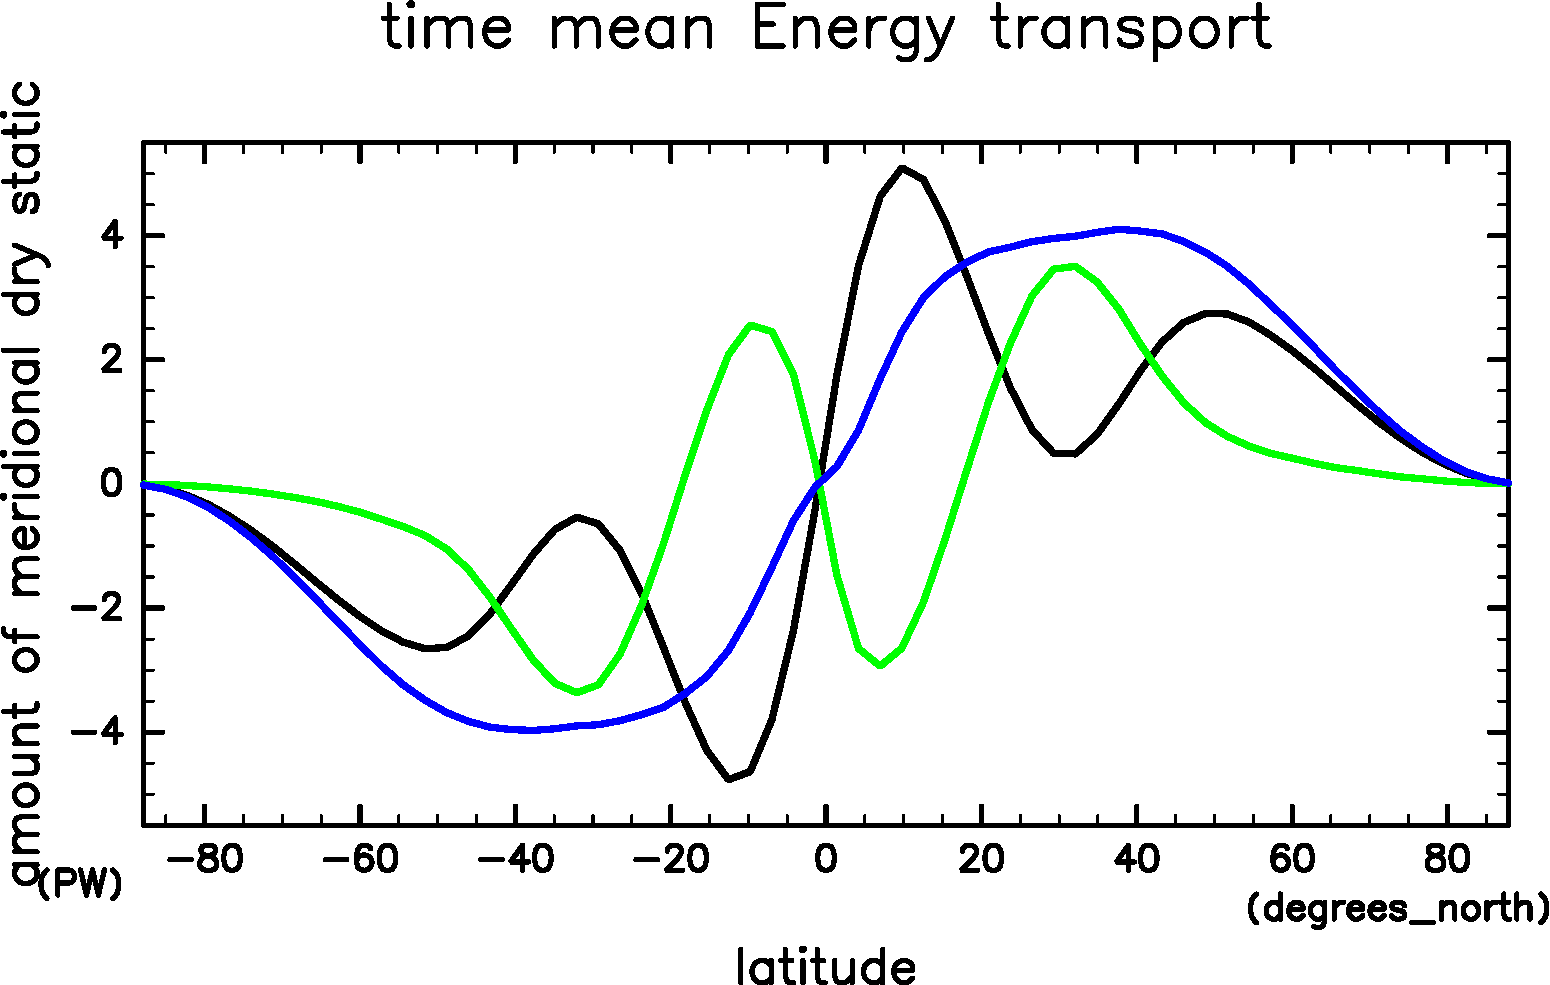
\includegraphics[width=\columnwidth]{S1366/EngyFlx,time=14600:14965-crop-rotate.pdf}
		\caption{\(S=1366\)}
	\end{subfigure}
	\begin{subfigure}{.17\textwidth}
		\centering
		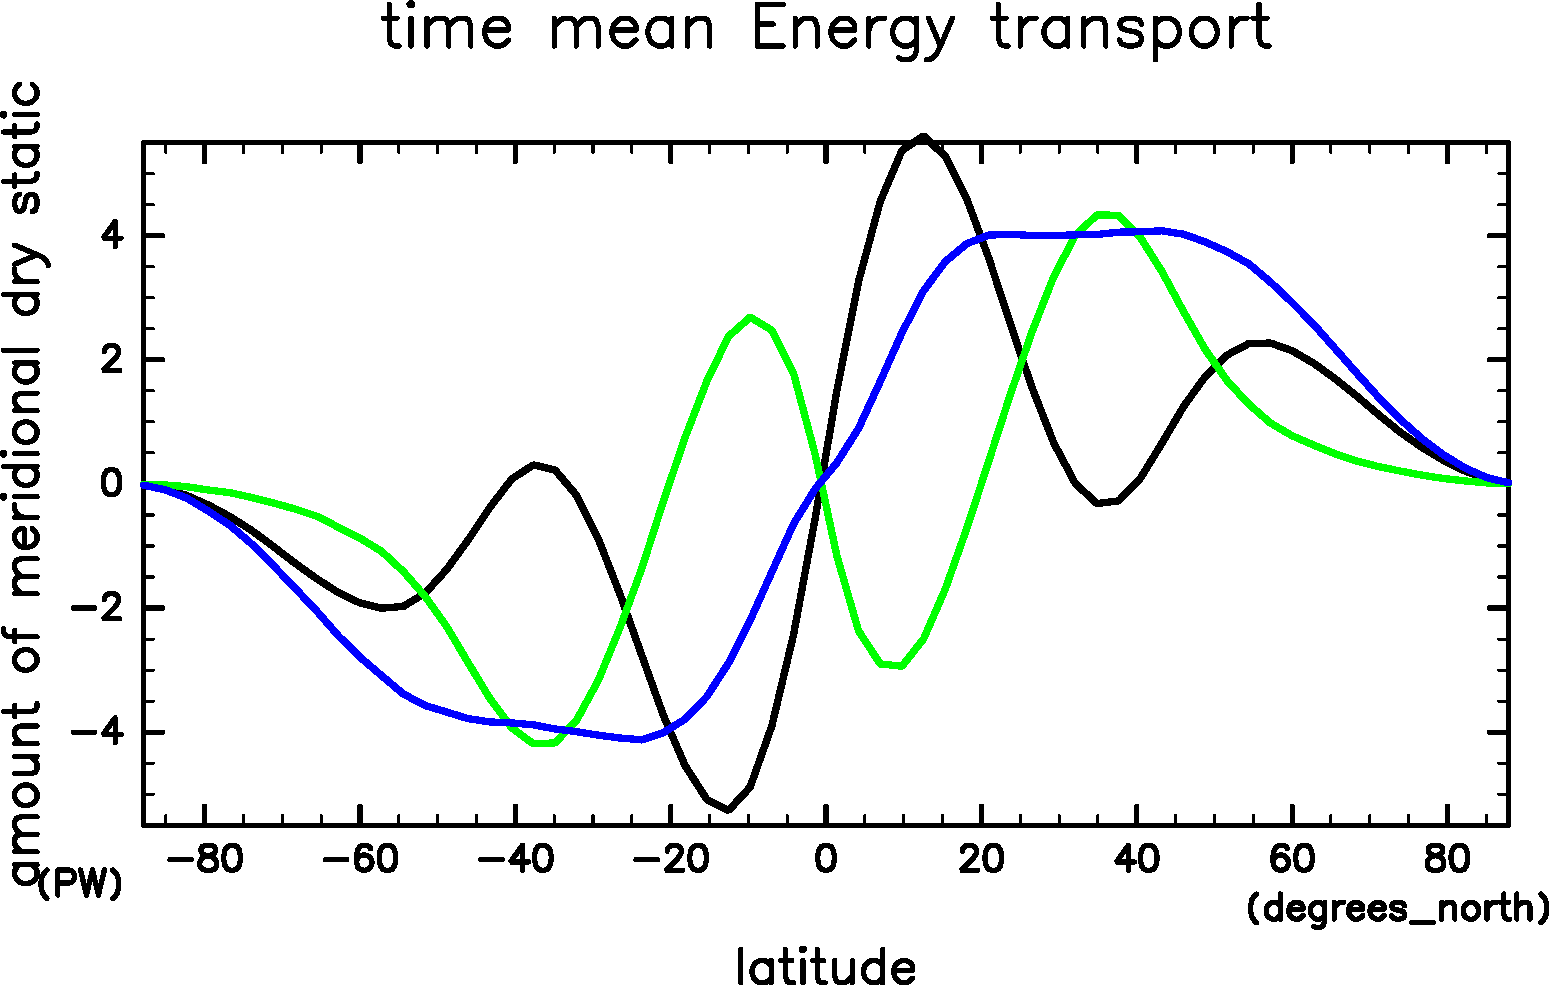
\includegraphics[width=\columnwidth]{S1500/EngyFlx,time=3650:4015-crop-rotate.pdf}
		\caption{\(S=1500\)}
	\end{subfigure}
	\begin{subfigure}{.17\textwidth}
		\centering
		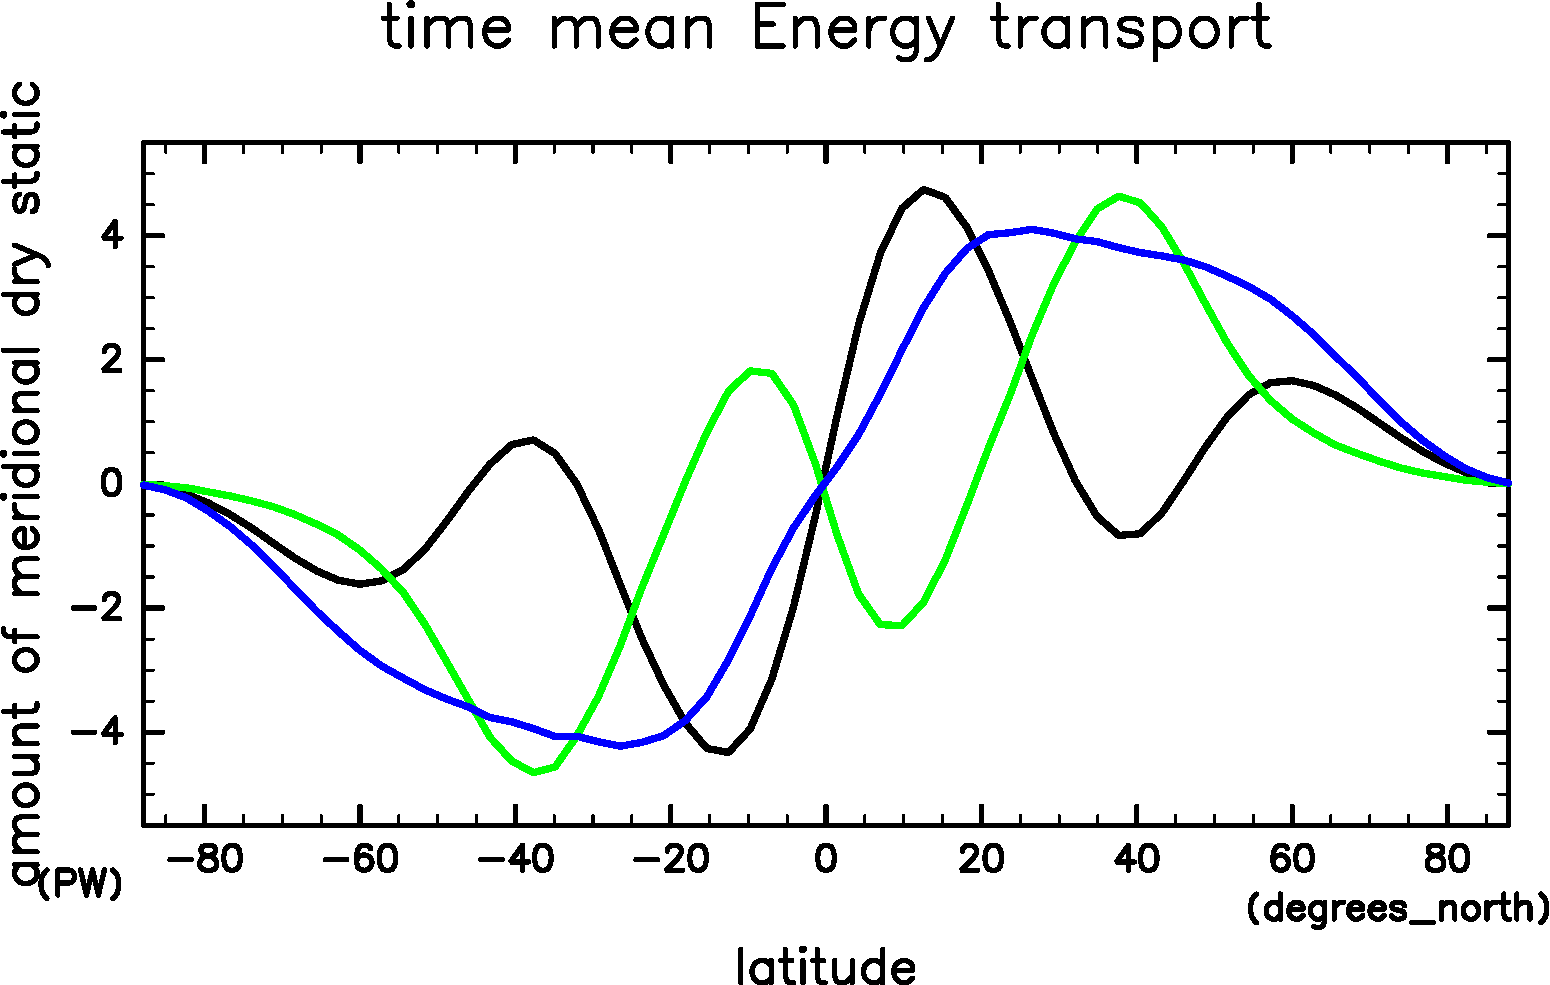
\includegraphics[width=\columnwidth]{S1600/EngyFlx,time=3650:4015-crop-rotate.pdf}
		\caption{\(S=1600\)}
	\end{subfigure}
	\begin{subfigure}{.17\textwidth}
		\centering
		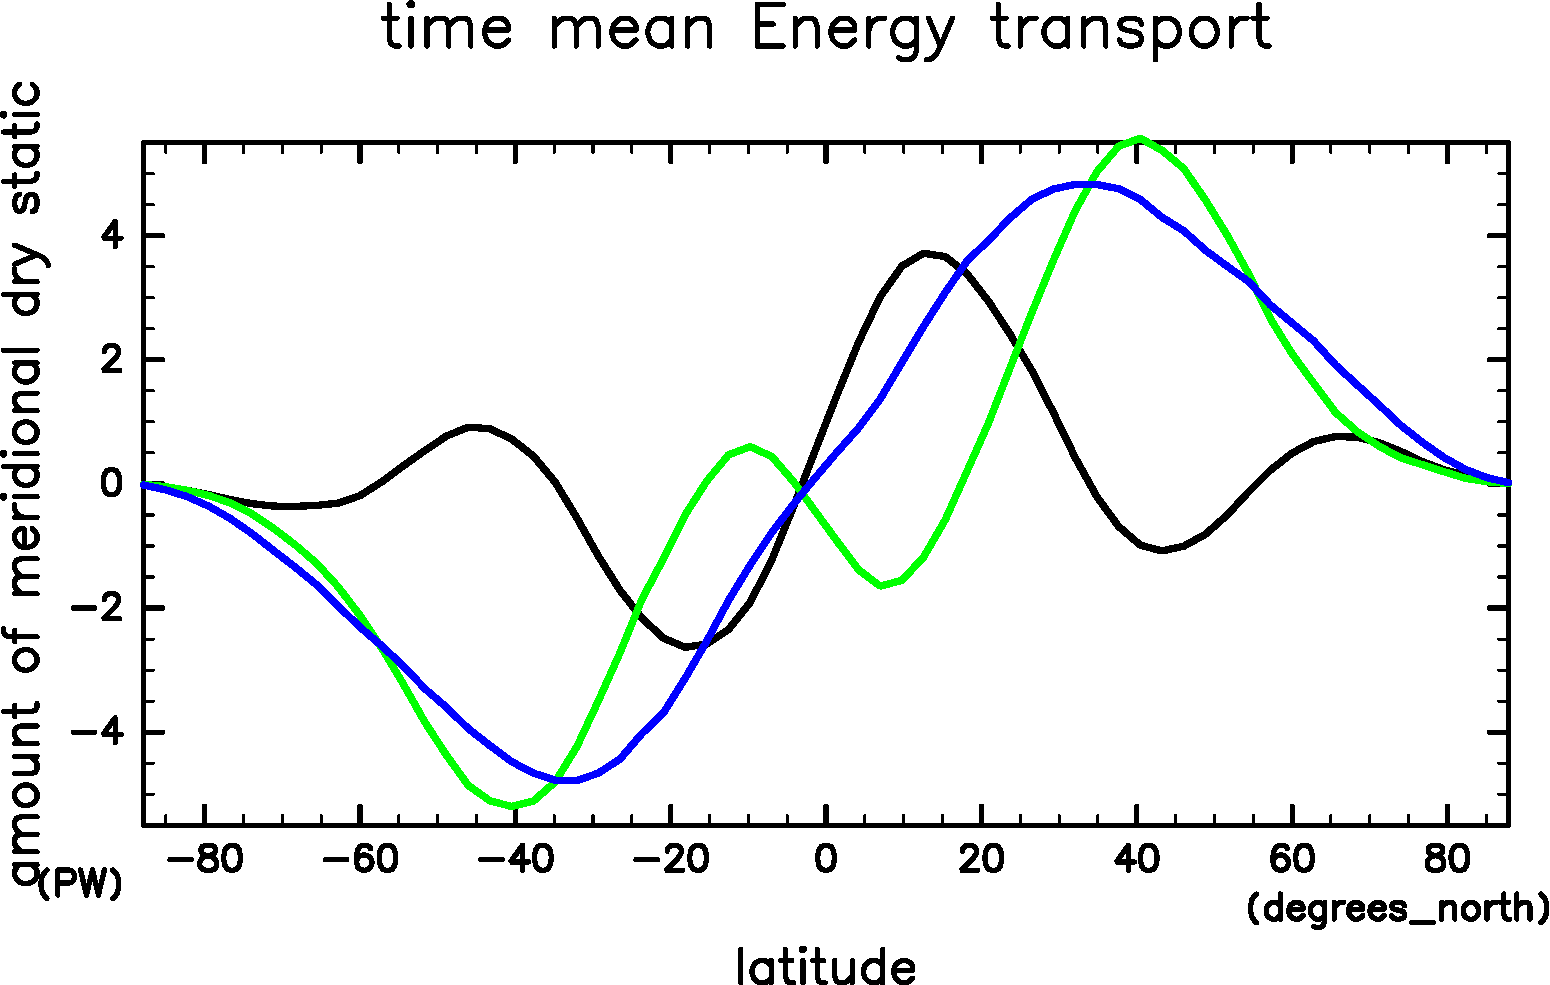
\includegraphics[width=\columnwidth]{S1800/EngyFlx,time=3650:4015-crop-rotate.pdf}
		\caption{\(S=1800\)}
	\end{subfigure}
	\begin{subfigure}{.17\textwidth}
		\centering
		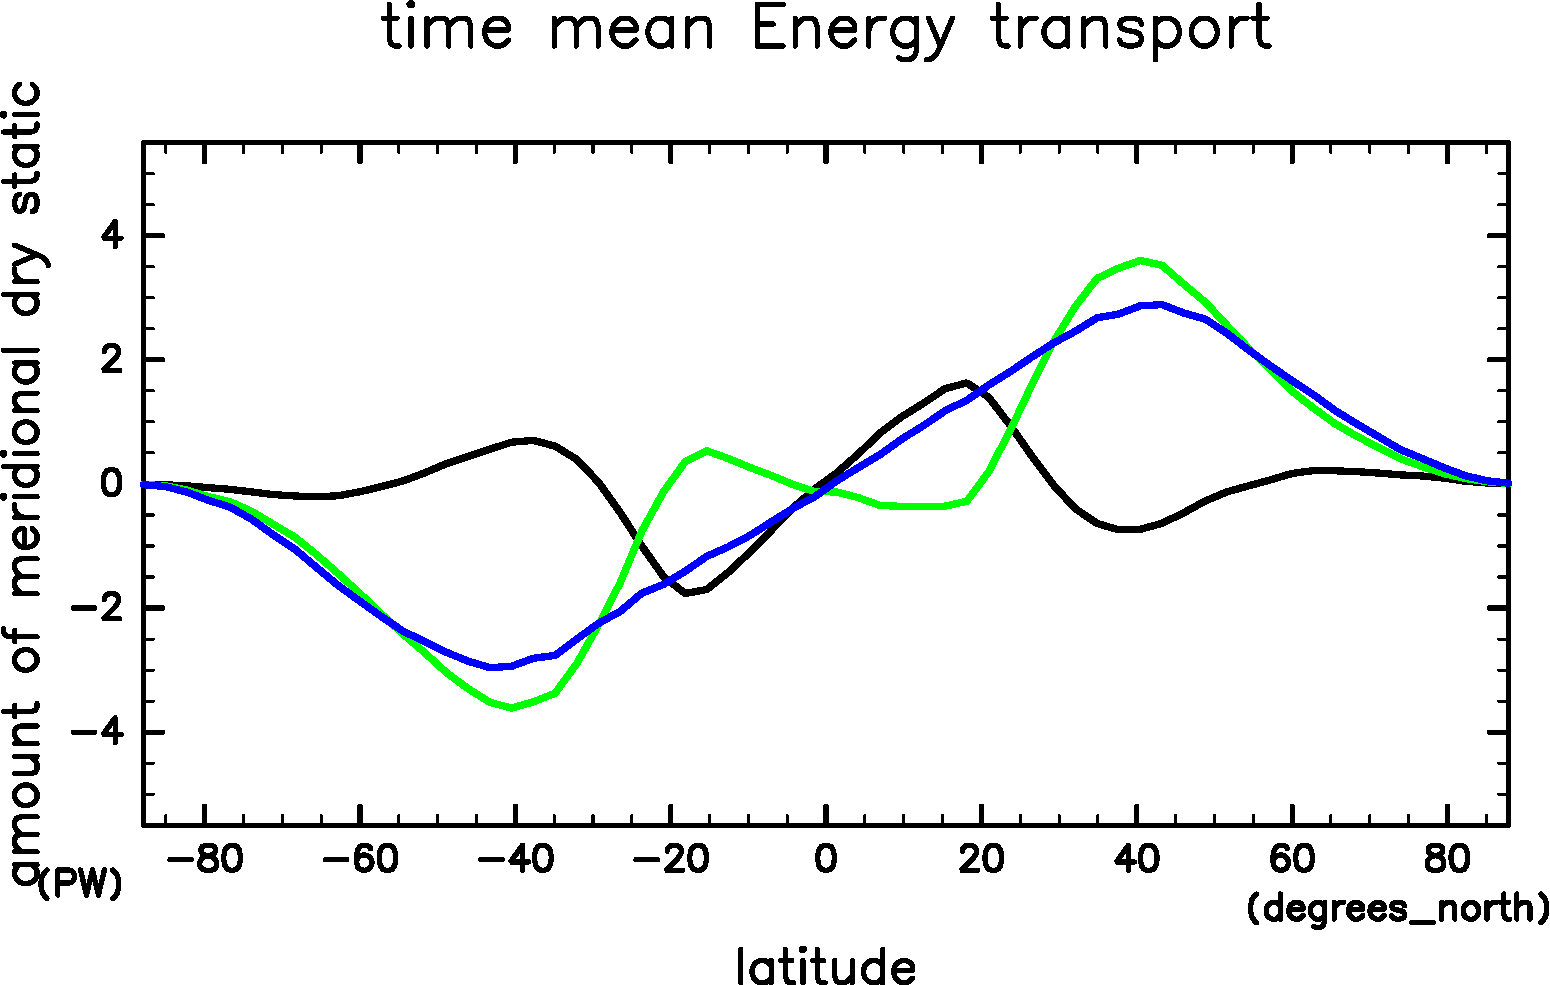
\includegraphics[width=\columnwidth]{S2000/EngyFlx,time=7300:7665-crop-rotate.pdf}
		\caption{\(S=2000\)}
	\end{subfigure}
	\caption{
		Meridional distributions of heat transports for all experiments. Blue lines are total transports,
		lime lines are latent energy transports, and black lines are dry static energy transports.
		Horizontal axis is latitude \([\hmu*{deg}]\) and vertical axis is amount of energy flux \([\hmu*{PW}]\).
	}\label{EnFlx}
\end{figure}

\enlargethispage{1cm}

\end{document}
